\newcommand{\NWtarget}[2]{#2}
\newcommand{\NWlink}[2]{#2}
\newcommand{\NWtxtMacroDefBy}{Fragment defined by}
\newcommand{\NWtxtMacroRefIn}{Fragment referenced in}
\newcommand{\NWtxtMacroNoRef}{Fragment never referenced}
\newcommand{\NWtxtDefBy}{Defined by}
\newcommand{\NWtxtRefIn}{Referenced in}
\newcommand{\NWtxtNoRef}{Not referenced}
\newcommand{\NWtxtFileDefBy}{File defined by}
\newcommand{\NWtxtIdentsUsed}{Uses:}
\newcommand{\NWtxtIdentsNotUsed}{Never used}
\newcommand{\NWtxtIdentsDefed}{Defines:}
\newcommand{\NWsep}{${\diamond}$}
\newcommand{\NWnotglobal}{(not defined globally)}
\newcommand{\NWuseHyperlinks}{}
\documentclass{article}
\usepackage{graphicx,color}
\begin{document}
\setlength{\parindent}{0in}
\title{\color{blue}Lab 2 Excercise P2.24}
\author{\color{blue}Frank Mock}
\date{\color{blue}September 18, 2011}
\maketitle
\section{Specification}

Exercise P2.24.
      
Make a bar chart to plot a data set of user intput.
Prompt the user to type in four names and measurements. 
Then display a bar graph. Make the bars horizontal for easier labeling.\\
\begin{tabular}{lc}
Name & Longest Span(ft) \\
Golden Gate & 4,200 \\
Brooklyn & 1,595 \\
Delaware Memorial & 2,150 \\
Mackinaw &3,800 
\end{tabular}
\section{Design}
\begin{enumeration}
\item Display message describing program
\item Define variables and setup the coordinate system. Prompt user for 
highest number in data set to assist setting up coordinate system
\item Prompt user to type four names and measurements and store in arrays
\item Display the bar graph
\end{enumeration}
\section{Analysis}
This exercise uses the authors graphics library ccc\_win.h available
from \footnote{www.wiley.com/college/horstmann}
To use this graphics library, you must include the header file ccc\_win.h 
into your program. Moreover, you need to supply the function ccc\_win\_main 
instead of main as the entry point to your program.
\begin{flushleft} \small
\begin{minipage}{\linewidth}\label{scrap1}\raggedright\small
\NWtarget{nuweb2a}{} $\langle\,${\it Display message describing program}\nobreak\ {\footnotesize {2a}}$\,\rangle\equiv$
\vspace{-1ex}
\begin{list}{}{} \item
\mbox{}\verb@@\\
\mbox{}\verb@        cwin << Message(Point(-5, -4), "Frank Mock");@\\
\mbox{}\verb@        cwin << Message(Point(-5, -5), "Lab 2.24");@\\
\mbox{}\verb@        cwin << Message(Point(-5, -6), "Graph Values Entered by User");@\\
\mbox{}\verb@@{\NWsep}
\end{list}
\vspace{-1.5ex}
\footnotesize
\begin{list}{}{\setlength{\itemsep}{-\parsep}\setlength{\itemindent}{-\leftmargin}}
\item \NWtxtMacroRefIn\ \NWlink{nuweb4a}{4a}.

\item{}
\end{list}
\end{minipage}\vspace{4ex}
\end{flushleft}
The first use of cwin is ignored on my machine but the machine I
used in class did not do this. To remedy this inconsistency, I prompt 
the user to see if they are ready. Their answer is not used. I choose
to create array data types to store user input. To make setting up
the coordinate system easier, I ask the user for the highest value
of the data set and use this in cwin's call to coord().
\begin{flushleft} \small
\begin{minipage}{\linewidth}\label{scrap2}\raggedright\small
\NWtarget{nuweb2b}{} $\langle\,${\it Define variables and setup the coordinate system}\nobreak\ {\footnotesize {2b}}$\,\rangle\equiv$
\vspace{-1ex}
\begin{list}{}{} \item
\mbox{}\verb@@\\
\mbox{}\verb@        //This prompt is not important and may not display on some machines@\\
\mbox{}\verb@        string not_used = cwin.get_string("Ready To Begin?(Y or N");@\\
\mbox{}\verb@        //Define variables@\\
\mbox{}\verb@        int measurement;@\\
\mbox{}\verb@        int measurments[4];@\\
\mbox{}\verb@        string names[4];@\\
\mbox{}\verb@        //set up coordinate system to be used@\\
\mbox{}\verb@        int highest = cwin.get_int("What is the highest value of the data set?");@\\
\mbox{}\verb@        cwin.coord(-10, 5, highest + 10, -10);@\\
\mbox{}\verb@@{\NWsep}
\end{list}
\vspace{-1.5ex}
\footnotesize
\begin{list}{}{\setlength{\itemsep}{-\parsep}\setlength{\itemindent}{-\leftmargin}}
\item \NWtxtMacroRefIn\ \NWlink{nuweb4a}{4a}.

\item{}
\end{list}
\end{minipage}\vspace{4ex}
\end{flushleft}
\\
\\
\\
I used a for loop to get the four names and measurements. The code
performs some validation utilizing a do-while loop and not allowing 
a number higher than what the user already inputed as the highest 
value of the data set. This ensures that the coordinate system will 
not be compromised by the values entered by the user. We can get 
information from the user using member functions from the GraphicWindow 
class. We can use get\_string for the name of the bridge and \verb|get_int| 
for it's length.
\begin{flushleft} \small
\begin{minipage}{\linewidth}\label{scrap3}\raggedright\small
\NWtarget{nuweb3a}{} $\langle\,${\it Prompt user for names and measurements and store in arrays}\nobreak\ {\footnotesize {3a}}$\,\rangle\equiv$
\vspace{-1ex}
\begin{list}{}{} \item
\mbox{}\verb@        @\\
\mbox{}\verb@        //Get Name and Number input from user@\\
\mbox{}\verb@        for(int count = 0; count <= 3; count++)@\\
\mbox{}\verb@        {@\\
\mbox{}\verb@                string name = cwin.get_string("Please type name");@\\
\mbox{}\verb@                names[count] = name;@\\
\mbox{}\verb@                do@\\
\mbox{}\verb@                {@\\
\mbox{}\verb@                measurement = cwin.get_int("Enter measurement:");@\\
\mbox{}\verb@                measurments[count] = measurement;@\\
\mbox{}\verb@                }while(measurement > highest);@\\
\mbox{}\verb@        }@\\
\mbox{}\verb@@{\NWsep}
\end{list}
\vspace{-1.5ex}
\footnotesize
\begin{list}{}{\setlength{\itemsep}{-\parsep}\setlength{\itemindent}{-\leftmargin}}
\item \NWtxtMacroRefIn\ \NWlink{nuweb4a}{4a}.

\item{}
\end{list}
\end{minipage}\vspace{4ex}
\end{flushleft}
I used a for-loop to interate through each array and draw the
users inputed data to the screen.
\begin{flushleft} \small
\begin{minipage}{\linewidth}\label{scrap4}\raggedright\small
\NWtarget{nuweb3b}{} $\langle\,${\it Draw bar graph info to screen}\nobreak\ {\footnotesize {3b}}$\,\rangle\equiv$
\vspace{-1ex}
\begin{list}{}{} \item
\mbox{}\verb@        @\\
\mbox{}\verb@        for(int count = 0; count <=3; count++)@\\
\mbox{}\verb@        {@\\
\mbox{}\verb@                string n = names[count];@\\
\mbox{}\verb@                int m = measurments[count];@\\
\mbox{}\verb@                Point topleft(0, count);@\\
\mbox{}\verb@                Point topright(m, count);@\\
\mbox{}\verb@                Point bottomleft(0, count - .5);@\\
\mbox{}\verb@                Line horizontal(topleft, topright);@\\
\mbox{}\verb@                Line vertical(topleft, bottomleft);@\\
\mbox{}\verb@                cwin << horizontal << vertical;@\\
\mbox{}\verb@                cwin << Message(Point(0, count), n);@\\
\mbox{}\verb@                horizontal.move(0, - .5);@\\
\mbox{}\verb@                vertical.move(m, 0);@\\
\mbox{}\verb@                cwin << horizontal << vertical;@\\
\mbox{}\verb@        }@\\
\mbox{}\verb@@{\NWsep}
\end{list}
\vspace{-1.5ex}
\footnotesize
\begin{list}{}{\setlength{\itemsep}{-\parsep}\setlength{\itemindent}{-\leftmargin}}
\item \NWtxtMacroRefIn\ \NWlink{nuweb4a}{4a}.

\item{}
\end{list}
\end{minipage}\vspace{4ex}
\end{flushleft}
\begin{flushleft} \small
\begin{minipage}{\linewidth}\label{scrap5}\raggedright\small
\NWtarget{nuweb4a}{} \verb@"p2_24.cpp"@\nobreak\ {\footnotesize {4a}}$\equiv$
\vspace{-1ex}
\begin{list}{}{} \item
\mbox{}\verb@@\\
\mbox{}\verb@@\hbox{$\langle\,${\it include files}\nobreak\ {\footnotesize \NWlink{nuweb4b}{4b}}$\,\rangle$}\verb@@\\
\mbox{}\verb@int ccc_win_main()@\\
\mbox{}\verb@{@\\
\mbox{}\verb@        @\hbox{$\langle\,${\it Display message describing program}\nobreak\ {\footnotesize \NWlink{nuweb2a}{2a}}$\,\rangle$}\verb@@\\
\mbox{}\verb@        @\hbox{$\langle\,${\it Define variables and setup the coordinate system}\nobreak\ {\footnotesize \NWlink{nuweb2b}{2b}}$\,\rangle$}\verb@@\\
\mbox{}\verb@        @\hbox{$\langle\,${\it Prompt user for names and measurements and store in arrays}\nobreak\ {\footnotesize \NWlink{nuweb3a}{3a}}$\,\rangle$}\verb@@\\
\mbox{}\verb@        @\hbox{$\langle\,${\it Draw bar graph info to screen}\nobreak\ {\footnotesize \NWlink{nuweb3b}{3b}}$\,\rangle$}\verb@@\\
\mbox{}\verb@        return 0;@\\
\mbox{}\verb@}@\\
\mbox{}\verb@@{\NWsep}
\end{list}
\vspace{-1.5ex}
\footnotesize
\begin{list}{}{\setlength{\itemsep}{-\parsep}\setlength{\itemindent}{-\leftmargin}}

\item{}
\end{list}
\end{minipage}\vspace{4ex}
\end{flushleft}
These are the include files needed for this program
\begin{flushleft} \small
\begin{minipage}{\linewidth}\label{scrap6}\raggedright\small
\NWtarget{nuweb4b}{} $\langle\,${\it include files}\nobreak\ {\footnotesize {4b}}$\,\rangle\equiv$
\vspace{-1ex}
\begin{list}{}{} \item
\mbox{}\verb@@\\
\mbox{}\verb@#include "ccc_win.h"@\\
\mbox{}\verb@@{\NWsep}
\end{list}
\vspace{-1.5ex}
\footnotesize
\begin{list}{}{\setlength{\itemsep}{-\parsep}\setlength{\itemindent}{-\leftmargin}}
\item \NWtxtMacroRefIn\ \NWlink{nuweb4a}{4a}.

\item{}
\end{list}
\end{minipage}\vspace{4ex}
\end{flushleft}
\section{Image of program p2\_24.exe running}
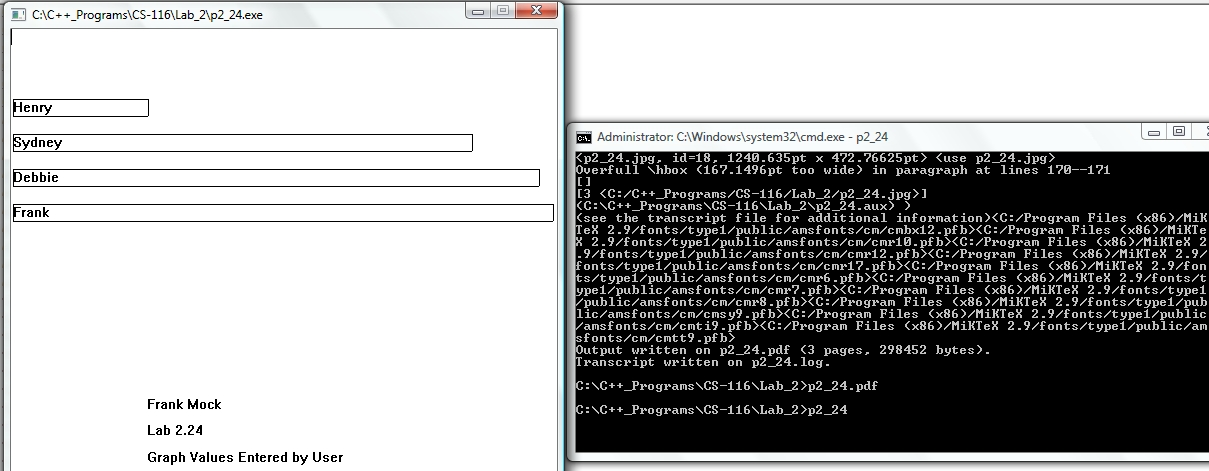
\includegraphics[width=18cm]{p2_24.jpg}
\end{document}